\documentclass[9pt,twocolumn,twoside]{../../styles/osajnl}
\usepackage{fancyvrb}
\journal{i524} 

\title{Weather Data Analysis}

\author[1]{Vishwanath Kodre}
\author[1]{Sabyasachi Roy Choudhury}
\author[1]{Abhijit Thakre}

\affil[1]{School of Informatics and Computing, Bloomington, IN 47408, U.S.A.}

\affil[1]{Corresponding authors: sabyasachi087@gmail.com, vkodre@gmail.com, athakre@gmail.com}

\dates{project-000, \today}

\ociscodes{Cloud, I524}

% replace this with your url in github/gitlab
\doi{\url{https://github.com/cloudmesh/classes/blob/master/docs/source/format/report/report.pdf}}


\begin{abstract}
The project aims to analyze any relationship between change in climate, geo- magnetic field and natural disasters with focusing on use of Hadoop Framework for data analysis and Ansible for automating deployment and monitoring.
\newline
\end{abstract}

\setboolean{displaycopyright}{true}

\begin{document}

\maketitle

\section{Introduction}

The study of environmental science and climatic changes around has been done for decades, the study
has always been predictive based on the past experiences and forecasting of the weather conditions
around us. With use of modern days technologies it determining the climatic changes and with analysis
done around it has helped human being to prepare and face the natural calamities. Though with current
equipment weather department has strengthen their arms but has not been able to be full proof and
many time its not been able to predict/ forecast the climatic changes effectively. The study of the
whether data and geo graphical changes is ongoing evolving process. Thus more and more researcher
needs modern days tools and technologies to leverage it and forecast more accurately.

\subsection{Objective}

The goal of this is to study the weather data and analyze the relationship between the geo graphical
changes such change in geo magnetic field and/or natural disaster. With use of Hadoop for distributed
data analysis aims to finds any pattern that might exists between these parameters. The course of the
analysis will also provides visualization of these parameters in order to identify any pattern in a more
intuitive way. By leveraging the power ansible for application deployment over cluster and monitoring
the application performance to determine scalability and throughput. The conclusion will be determine
by establishing any existing pattern, analysis done over it and by visualizing it.

\section{Data Sources}

Weather data has been recorded since 19th century. This data can be used to estimate climate changes
and forecasting. The same data can be can be used to find any existing pattern with natural disasters.
Following sources has been compiled for weather, natural disaster and geo magnetic fields.
\begin{itemize}
\item Weather-Data\cite{Weather-Data}
\item Natural Disaster\cite{Disaster-List-Data}
\item Geo Magnetic Field\cite{Geo-Magnetic-Data}
\end{itemize}

\section{High Level Design}

The design of the application is thought of leveraging power of Hadoop as main processing unit of
analysis with deployment on the cluster environment where application requires multiple processing
units for execution, database for persistence and visualization tools for graphical outputs.
\begin{figure}[htbp]
\centering
\fbox{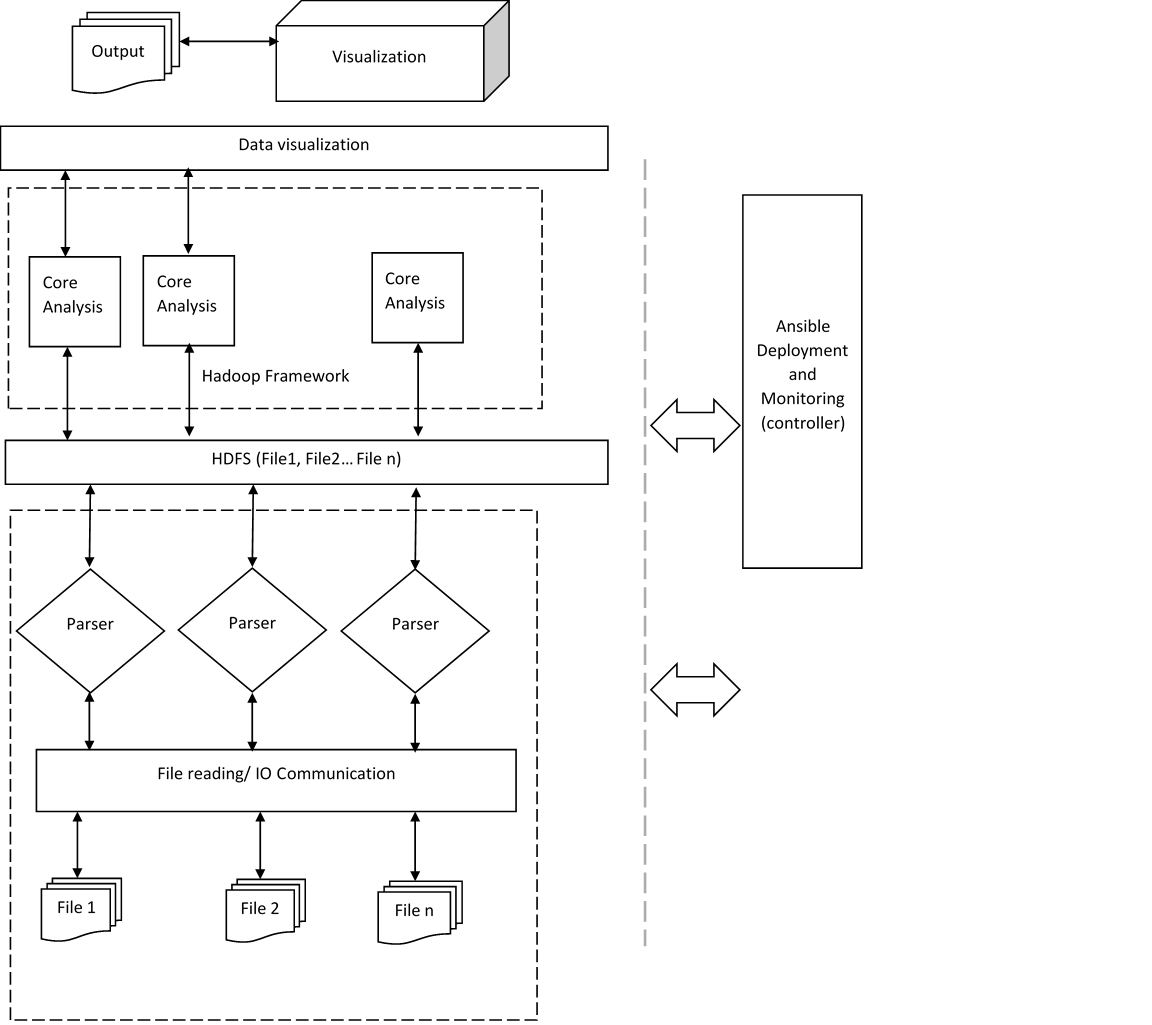
\includegraphics[width=\linewidth]{images/weather_analysis_architecture}}
\caption{Architecture}
\label{Reference:false-color}
\end{figure}
The project is divided into following steps:

\begin{itemize}
\item Data cleaning and persistence - The raw data cannot be use directly for analysis. First data has to be parsed and required parameters will be extracted. Then this extracted data will be dumped into a NoSql database.
\item Core Analysis Program - Core analysis program will be responsible for figuring out any hidden patterns between aforesaid parameters. Program will compare natural disasters occurred, geo-magnetic orientation and climate data
set on a given location and duration and compute relationship between them. The program will be an
MapReduce implementation and is the heart of the application. The program will be executed through
Hadoop framework. Hadoop will execute the program in a distributed manner.
\item Deployment and Monitoring - The application needs multiple processing units and monitoring system. Ansible will be used for deployment and manage nodes for program execution.Ansible will be responsible for following tasks
i)   Deployment and configuration of Hadoop on the multiple nodes.
ii)  Starting Hadoop servers, inserting/reading data.
iii) Execution of the commands to run the analysis using Hadoop to filter the input data and write
response to HDFS or some output file.
iv)  This output can be then passes to the visualization step as the input data.
\item Visualization - Finally once the programs completes execution, using the scikit-tool or other visualization tool
kit and the output file, graphs and patterns depicting the relationship can be plotted more intuitive representation.
\item BenchMarking - The application can be benchmarked for the scalability by addition more nodes and checking the
performance for strong scaling. The report will be represented in tabular format.
\end{itemize}


\section{Data Curation}
Getting data ready is the very first and basic step for analysis. We have chose NCDC as our source of data. NCDC exposes few rest apis for accessing weather data. Following will give you a brief understanding on the apis used for getting the required data.
\begin{itemize}
\item I) Datasets : This groups data into monthly daily , yearly pattern. There are eleven different datasets. We will be choosing GSOM (Global Summary Of Monthly) as our primary datasets. (URL : https://www.ncdc.noaa.gov/cdo-web/api/v2/datasets ,Attributes : GSOM). For this project we will use GSOM only.	
\item II) Data Categories: This groups data into data category like Temperature, Pressure etc. We will consider only few. ( URL : https://www.ncdc.noaa.gov/cdo-web/api/v2/datacategories, Attributes : "TEMP" (Air Temperature) , "PRES" (Pressure) , "EVAP" (Evaporation) and "VELOCITY" (Velocity) ). For our project we will be using PRCP, SNOW, TMAX, TMIN and TAVG.
\item III) Data Types: This group Data Categories into further smaller sub types. (URL : https://www.ncdc.noaa.gov/cdo-web/api/v2/datatypes?datasetid=GSOM&datacategoryid=TEMP , Attributes : "TAVG" (Average Temperature), "TMAX" (Maximum Temperature) and "TMIN" (Minimum Temperature)    ) Other Data Categories does not have sub type.
\item IV) Location Categories: This groups data in terms of location. (URL:https://www.ncdc.noaa.gov/cdo-web/api/v2/locationcategories , Attributes : "CITY" , "CLIM_DIV" (Climate Division), "CLIM_REG" (Climate Region) , "CNTRY" (Country) ,"ST" (State)). For this project we will be downloading data for India only.
\item V)  Location: Groups data in terms of country, state etc. (URL : https://www.ncdc.noaa.gov/cdo-web/api/v2/locations?locationcategoryid=CNTRY, Attributes : "FIPS:IN" (INDIA) , "FIPS:IO" (Indian Ocean))	
\item VI) Station : This collects stations details based on the location id. (URL : https://www.ncdc.noaa.gov/cdo-web/api/v2/stations?locationid=FIPS:IN , Attributes: ids , mindate and maxdate). All of the stations details will be collected.	
\item VII) 	Data : This collects actual weather data for the given stationId, start_date and end_date. (URL : https://www.ncdc.noaa.gov/cdo-web/api/v2/data?datasetid=GSOM&stationId=GHCND:IN1NCBC0005&startdate=1970-10-10&enddate=1971-10-10). Since the project only requires only 5 attributes, further filter is applied while invoking the API. The data received will be saved into database. 
\end{itemize}

\subsection{Collecting Data}
NCDC uses token based authentication for security and with each token , no more than 10,000 hits are allowed per day. Well 10,000 seems huge but truly its not. We have targeted one country (India) and 5 attributes chiefly precipitation, snow, maximum temperature, minimum temperature and average temperature for each month. Total number of weather data stations in the country is around 3500 and each station has a data range of 30 to 50 years. This leads to a total of 100,000 hits or more. To handle this, we need to load data incrementally, i.e. the curation program should have the ability to resume the download from the last save point. Before we dive more into logical section , lets first see the technology stack for data collection.

\subsection{Technology Stack}
We have considered python , Apache thrift and Apache Hbase for data curation step. We will be covering a short introduction of the steps to configure the system, before diving into the core logic of curation. Since we are going to use Apache Hadoop for our analysis purpose, Hbase comes as a natural choice of NoSql database. Java is the default language for both Hadoop and Hbase. So now the question is how to connect to Hbase using python and the solution is Apache Thrift or thrift. Thrift is a library from apache which generates hbase client. Thrift supports many third party languages including python. The following steps will be required to install thrift first.
\subsubsection{Install Apache Thrift \cite{thrift-python-install}}
\begin{itemize}
\item 1) Download Thrift from "http://redrockdigimark.com/apachemirror/thrift/0.10.0/thrift-0.10.0.tar.gz".
\item 2) Extract the file and run ./configure.
\item 3) Execute sudo make install or simply make to generate the binaries. If using make, the thrift binaries has to put into path manually (can be found under compiler/cpp/).
\item 4) After thrift is available in path , it can be tested by running "thrift --version".
\item 5) Then the python module has to be created to be used within python. To do this download "https://github.com/apache/hbase/blob/master/hbase-thrift/src/main/resources/org/apache/hadoop/hbase/thrift/Hbase.thrift" file.
\item 6) Then execute "thrift --gen py <path/to/Hbase.thrift>". This will generate "gen-py" folder.
\item 7) Add this folder to python path by export PYTHONPATH=<path/to>/gen-py/:$PPYTHONPATH.
\end{itemize}
For details you can check \href{https://acadgild.com/blog/connecting-hbase-with-python-application-using-thrift-server/}{Installation} steps.Installation of Hbase will be discussed later along with Hadoop.
Now thrift is ready to use. Execute "/hbase thrift start" to start the thrift server. Hbase has to be started separately.
\subsubsection{Install Happybase \cite{happybase-install}}
Happybase is a wrapper program written on thrift to facilitate data access layer in python in a more readable and swift way. Rather than using thrift client directly we will be using happybase python module. To install happybase run "pip install happybase". 
Once done test the python library by running the following test code 
\begin{lstlisting}[label=python,caption=Connect-Hbase]
import happybase as hbase				

connection = hbase.Connection('localhost')
print connection.tables()
\end{lstlisting}

Once happybase, thrift and hbase is functional, we are ready to download our weather data. Weather data download is divided into two steps 1) Getting weather stations details for a given country and 2) Getting Weather data for a given station. Lets see them individually :
\begin{itemize}
\item Download Weather Stations - To consume rest services we have used python's inbuilt request response module.  Let us walk you through the code. We have two main python script one for data access and another for rest consumption. "stations_dao.py" is for accessing table "wda_stations" in hbase. The functions are self explaining and hence will not be repeated here. "weather_services.py" is for consuming NCDC rest services. To load all stations , contd...

\end{itemize}

\section{Deployment Using Ansible}

Ansible is open source automation tool. It can be used for deployment of software, configuration  management and automation in the execution of application.
It also serves for monitoring of the state of the application. As per current state of our project we have used ansible for deployment of software in our project.
The script deploys Java, Hadoop, Hbase on the independent clusters. It also configures the properties in the key files.

\subsection{Inventory Configuration}

Inventory file contains the list of hostname or nodes that can be accessible by ansible. These nodes are then used in the script for deployment and configuration.
In the current project chameleon server nodes were created and configured. These IP address can be changed dynamically. This file can also contain the group inside
Which multiple ip can be configured.

[weatherCluster]
129.114.33.165 ansible_ssh_user=cc
129.114.33.179 ansible_ssh_user=cc
129.114.33.109 ansible_ssh_user=cc

\subsection{Playbook}

Playbook works on mentioned host of group. It mentions the roles those will be operated on each of the host. The main.yml  inside the task folder within each roles will be applied to
The cluster.

---
- hosts: weatherCluster
  remote_user: root
  roles:
    - master
    - hadoop
    - hbase
    — hdfs

\subsection{Roles}

% Bibliography

\bibliography{references}
 


\end{document}
